\documentclass[10pt]{beamer}

\usetheme[progressbar=frametitle,titleformat=allsmallcaps]{metropolis}
\usepackage{appendixnumberbeamer}

\usepackage{booktabs}
\usepackage[scale=2]{ccicons}

\usepackage{pgfplots}
\usepgfplotslibrary{dateplot}

\usepackage{xspace}
\newcommand{\themename}{\textbf{\textsc{metropolis}}\xspace}

\title{Modelling and analysis of dice-based stochastic games}
\subtitle{Level 4 Individual Project}
% \date{\today}
\date{}
\author{Lewis Dyer}
\institute{University of Glasgow}
% \titlegraphic{\hfill\includegraphics[height=1.5cm]{logo.pdf}}

\begin{document}

\maketitle

\begin{frame}{Challenges in game balance}
\begin{itemize}
\item Games exhibit \alert{emergent complexity}
\item Many games use random elements, most notably \textbf{dice}
\item Playtesting is time-consuming and resource-intensive... and fundamentally flawed
\item Some sort of automation would be hugely beneficial
\end{itemize}
\end{frame}

% \begin{frame}{The scale of game complexity}
% %Simple optimal strategies are dull, complex ones are interesting but hard to model. Somewhere in the middle...

% \includegraphics[width=\textwidth]{images/optimal_complexity.pdf}

% \end{frame}

\begin{frame}{Why model checking?}
\begin{itemize}
    \item Automated results (can limit playtesting)
    \item Easy game parameterisation
    \item Can \alert{exhaustively consider all possibilities} throughout a game
\end{itemize}
\end{frame}


\begin{frame}{Model hierarchy}

\begin{figure}
\centering
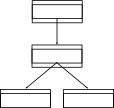
\includegraphics[height=0.7\textheight]{images/model_hierarchy.pdf}
\end{figure}

\end{frame}

\begin{frame}{Case Study 1: Shut the Box}
%Explain basic rules (maybe with visual aid?), explain basic strategies.
\begin{columns}[T] 
\begin{column}{0.5\textwidth}
\begin{itemize}
    \item Roll dice, cover boards
    \item Aim to maximise sum of covered boards
    \item The "high-board" strategy
\end{itemize}
\end{column}
\begin{column}{0.5\textwidth}
\includegraphics[width=\textwidth]{images/shut_the_box.jpg}
\end{column}
\end{columns}

\end{frame}

\begin{frame}{Strategy comparison}
%Show the big fancy graph, explain why this indicates Shut the Box is badly designed (optimal strategy too similar to high-board one)

\includegraphics[width=\textwidth]{images/stb12_2d6_prob_score.pdf}
\end{frame}

\begin{frame}{Case Study 2: Liar's Dice}
%Again basic rules, show how partial observability impacts things.
\begin{columns}[T] 
\begin{column}{0.5\textwidth}
\begin{itemize}
    \item Make bids, challenge other player's bids
    \item Players in the lead have more information
    \item Potential for snowballing
\end{itemize}
\end{column}
\begin{column}{0.5\textwidth}
\includegraphics[width=\textwidth]{images/Perudo.jpg}

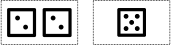
\includegraphics[width=\textwidth]{images/different_information.pdf}
\end{column}
\end{columns}
\end{frame}

\begin{frame}{Game tree construction}
%Show how to construct a game tree, give results for basic strategies, show snowball effect.
\begin{figure}
    \begin{overprint}
    \onslide<1>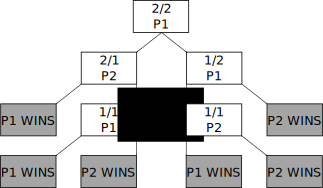
\includegraphics[width=\textwidth]{images/2_dice_game_tree.pdf}
    \onslide<2>\includegraphics[width=\textwidth]{images/2_dice_game_tree_rates.pdf}
    \end{overprint}
\end{figure}
%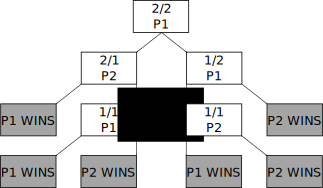
\includegraphics[width=\textwidth]{images/2_dice_game_tree.pdf}
\end{frame}

\begin{frame}{Case Study 3: 26.2}
%Again basic rules, impact of concurrency

\begin{columns}[T] 
\begin{column}{0.5\textwidth}
\begin{itemize}
    \item Choose how many dice to roll each turn
    \item Trade-off between going farther and going bust
    \item Simultaneous decision making exacerbates this trade-off
\end{itemize}
\end{column}
\begin{column}{0.5\textwidth}
\includegraphics[width=\textwidth, height=\textheight]{images/26point2.jpg}
\end{column}
\end{columns}
\end{frame}

\begin{frame}{Differentiating between strategies}

\begin{table}[h]
    \centering
    \begin{tabular}{lll}
    \hline
    P1 strategy                                                      & P2 strategy                 & Probability of P1 winning game \\ \hline
    4-dice                                                           & \multicolumn{1}{l|}{2-dice} & 0.8427                         \\
    3-dice                                                           & \multicolumn{1}{l|}{4-dice} & 0.5630                         \\
    hybrid                                                           & \multicolumn{1}{l|}{3-dice} & 0.5536                         \\
    hybrid                                                           & \multicolumn{1}{l|}{4-dice} & 0.5685                         \\
    \begin{tabular}[c]{@{}l@{}}optimal against\\ 3-dice\end{tabular} & \multicolumn{1}{l|}{3-dice} & 0.5608                        
    \end{tabular}
    \end{table}

Strategies are \alert{not sufficiently differentiable!}

\end{frame}



\begin{frame}{Conclusion}

\begin{itemize}
    \item Model checking viable for game design, including hidden information/concurrent games
    \item Model size is a key bottleneck for now
    \item Improve methods for comparison between strategies
\end{itemize}

\end{frame}

\begin{frame}[standout]
    Thanks for watching!
\end{frame}

\end{document}
